%build with pdflatex to include frontpage

% This is the main report file
\documentclass{acm_proc_article-sp}
\usepackage[utf8]{inputenc}
\usepackage{listings}
\usepackage{pdfpages}
\begin{document}

\title{02321 Hardware/Software programming Jan 11}
\subtitle{[Technical University of Denmark]
%\titlenote{This report should also be available online at \texttt{www.retrospekt.dk/02228report}}
}

\numberofauthors{2}
\author{
\alignauthor 
Kim Rostgaard Christensen\\
       \email{s084283@student.dtu.dk}
\alignauthor 
Morten Hillebo
       \email{s072923@student.dtu.dk}
}

%formal frontpage
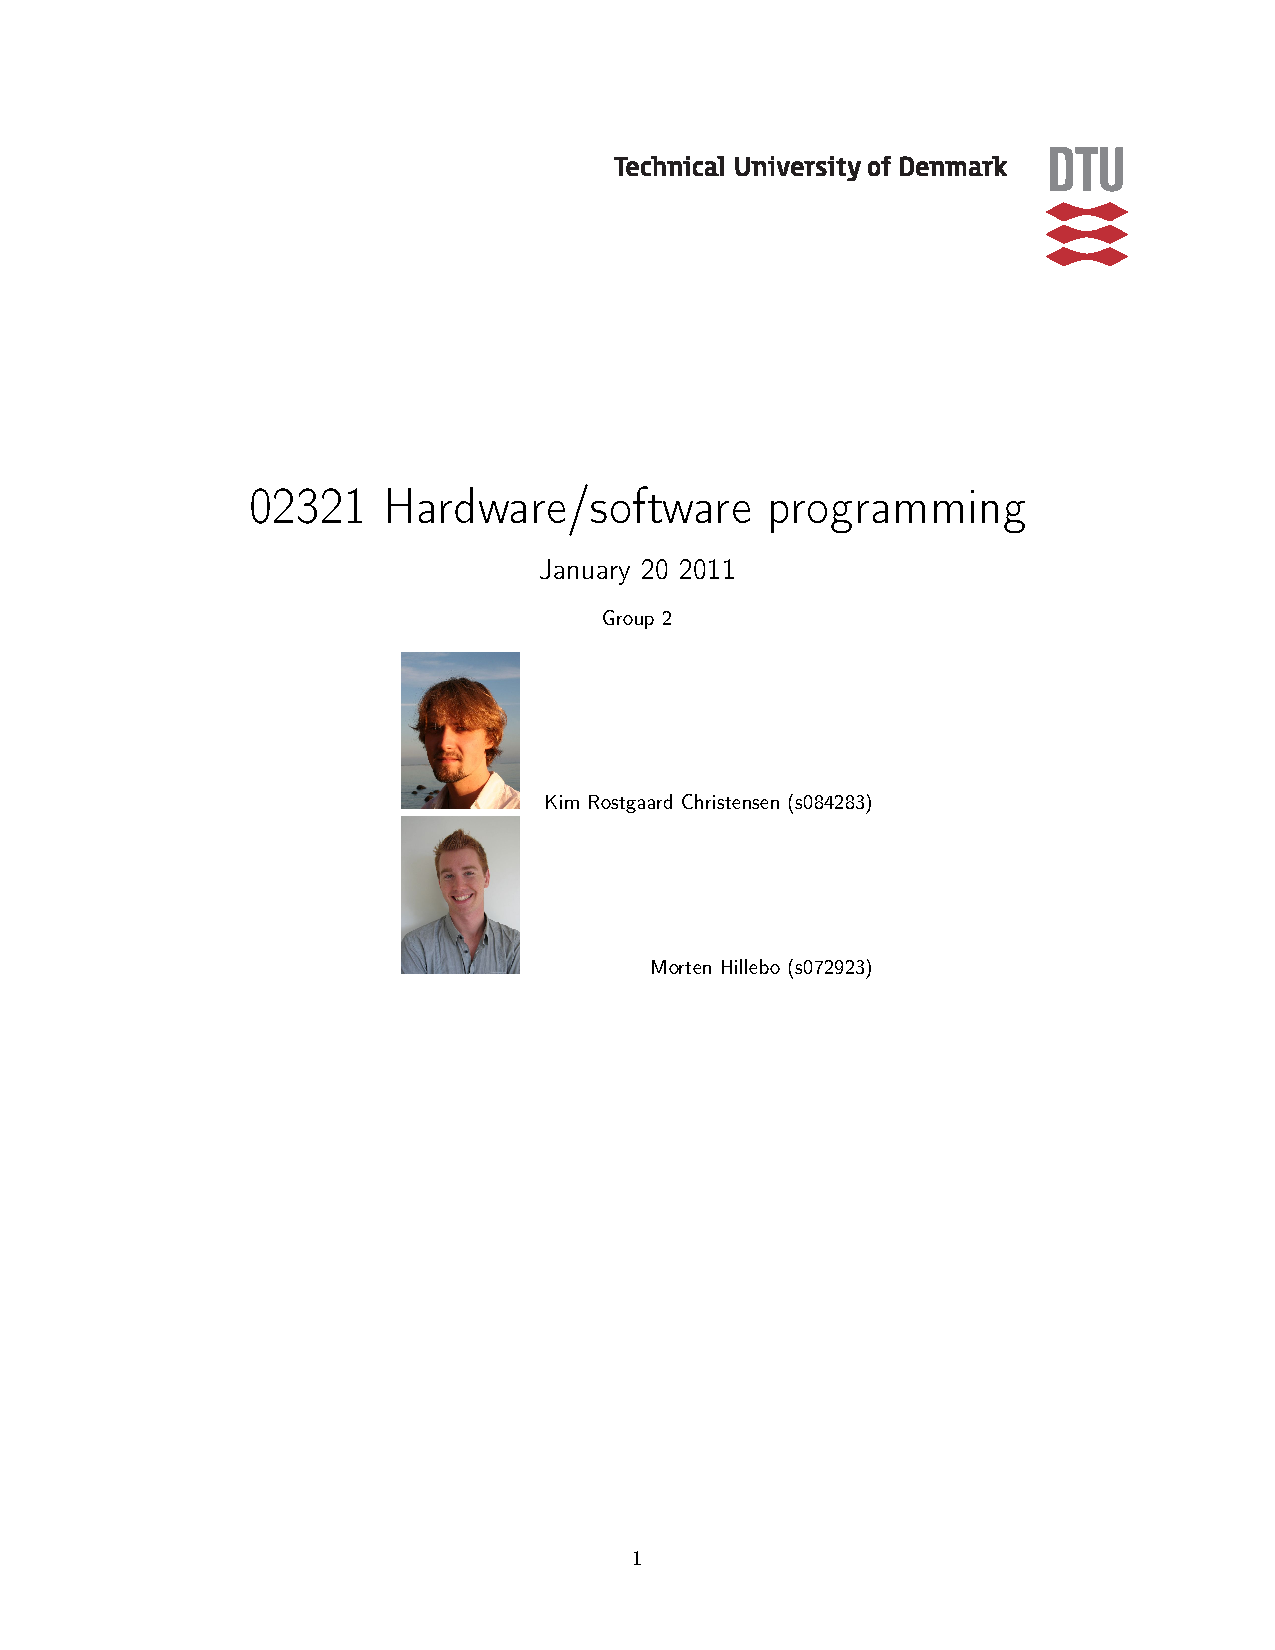
\includepdf{frontpage.pdf}

%\maketitle

\begin{abstract}
%Abstract; A brief summary of all of the report including the conclusion section
%but excluding the acknowledgements, references and any appendixes.
This project will cover the implementations of the LC-3 computer introduced in the book "Introduction to computing systems"\cite{patt2000introduction} by Patt And Patel, and the classic video game Snake to a FPGA-board. 
The goal has been to implement as many aspects of the computer as possible. 
Furthermore implement the game on the FPGA-board so no help was needed by any additional computer resources.
\end{abstract}

\section{Introduction}
\label{sec:introduction}

%TODO explain what the snake game is - briefly
The video snake game was first released in the mid 1970's and has since become a true video game classic. 
The game play involves navigating a snake around on the screen in search for food. 
The food will make the snake gain body length and increment the game score. 
The walls and eventual hurdles in the play area will cause the snake to die if collided.
This project is about developing and implementing the snake game on the LC3 processor. 

\begin{figure}[h]
\centering
%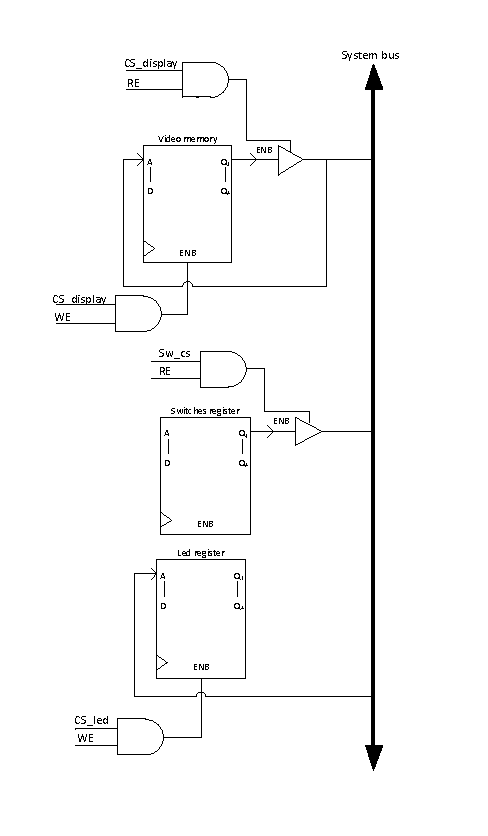
\epsfig{file=fig/system.eps, width=3.0in}
\includegraphics[scale=0.2]{img/FPGAForRepport.jpg} 
\caption{System architecture}
\label{fig:architecture}
\end{figure}

The overall architecture of the system involves the FPGA that implemented with the LC3 is the main computer in the system, a PC for programming the FPGA and a monitor for visualising the game that runs on the FPGA. 
The game navigation is controlled by using the buttons on the DIO4 board connected to the FPGA or a keyboard.

\section{Requirement specification}
The snake game requirement specification is split in two sections. The minimal implementations which is the logic needed, to provide a functional implementation of the game.
The second section suggests improvements and enhancement to implementations that will add visual improvements or additional game logic to make better game play. 

\subsection{Minimal implementation}
The minimal implementation requirements involves the basic elements and features of the game. The area where the snake can move around will be contained within a perimeter marked with wall elements. The Snake consists of two basic elements, a head and a number of body elements, where the body elements must follow the snake's head. When the snake head collides with the wall or its own body elements the snake will die, and the game will restart. Food elements will be placed within the wall perimeter and if the snake is navigated to a food element the snake will "consume" the food element and it's body elements is incremented resulting in an longer snake length and points added to the game score. The navigation of the snake is done directly on the FPGA using the buttons.

%\begin{itemize}
%\item Basic game logic (snake control, food consumption and growth)
%\item Basic game display (level and snake by blocks) 
%\item Simple levels
%\end{itemize}

\subsection{Enhancements}
An enhancement could be to implement a keyboard as the navigation device in the game logic and in the underlying implementation of the LC-3. 
Additional visual game enhancements by implementing advanced graphics with more colors, animated sprites and updating graphic elements of the snake and game environment. 
More complex game levels, snake speed increment and maybe even multi player possibilities. 

%\begin{itemize}
%\item Keyboard navigation on the board 
%\item Enhanced game display (sprites instead of blocks) 
%\item Enhance game play various objects (power-ups)  
%\item Complex levels with obstacles
%\item Multi player functionality 
%\end{itemize}

\section{Design}
There are different paths when it comes to the implementation of the game. The game can, for instance, run partially on a PC or completely on the LC3 - we have aimed for the latter.

There are two parts of the design; the hardware and the software.
\subsection{Hardware design}
The hardware part of the system consists of a black box processor that is connected to a system bus. This bus is then connected to the individual components as shown in figure \ref{fig:system}. 
\begin{figure}[h]
\centering
%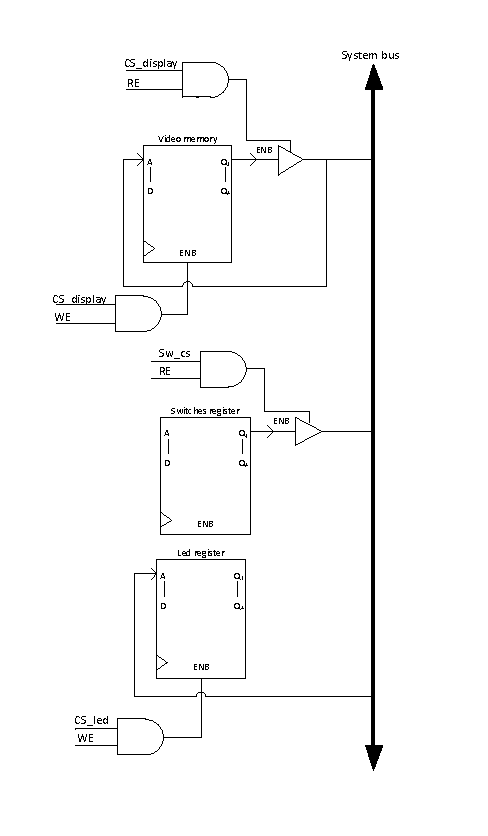
\epsfig{file=fig/system.eps, width=3.0in}
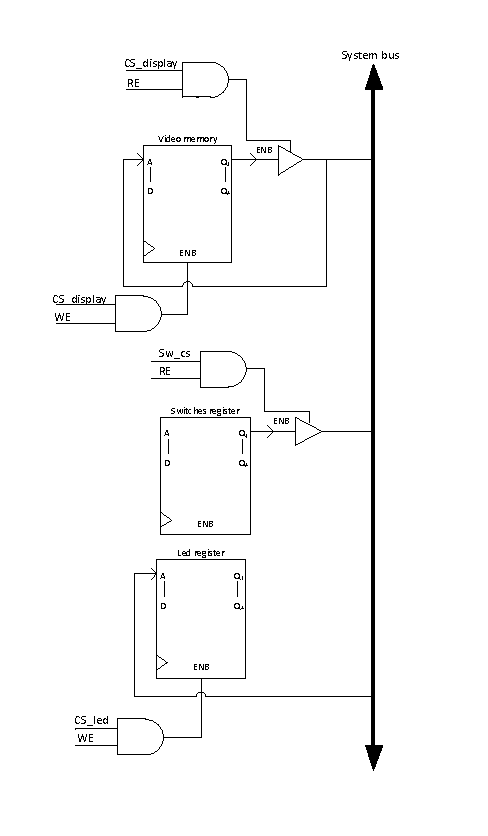
\includegraphics[width=3.5in]{fig/system.pdf}
\caption{Part of the system design}
\label{fig:system}
\end{figure}
Every individual component connected to the bus has its out port separated from the bus by a tri-state buffer that removes the data from the bus when the enable signal is not asserted.

The enable signal is a logical and gate with the inputs chip select signal and read enable or write enable signal from the processor. The chip select is an individual signal that is defined for each component. The signal is set to logic '1' when the address that has been reserved to the device is accessed.

The devices connected to the bus is currently the following
\begin{itemize}
	\item UART
	\item Main memory
	\item Custom tile video memory
	\item Led
	\item Push buttons
	\item Input switches
\end{itemize}
The tile video memory is the template from \cite{chu2008fpga} with a modified ROM for generating the characters.

The UART is a bi-directional serial connection between the PC and the FPGA board dedicated to program upload initially.

\subsubsection{Memory mapping}
In order to provide access from the programming language to the various I/O devices available, an interface is needed. This is in the form of a memory map, where certain areas of the memory is significant - or reserved. As the name would suggest, these memory areas are mapped onto the registers of the corresponding devices. A list of the I/O mappings can be found in table \ref{table:io_mappings} and \cite{patt2000introduction}. The memory locations where the registers reside is considered to be holes in memory, as these cannot be accessed due to the routing that happens in memory map.
\begin{table}[h]
\centering
    \begin{tabular}{ | l | l | l |}
    \hline
     Register & Memory address \\ \hline 
    \hline
    Video memory           & xE000  \\ \hline
    Stdin Status Register  & xFE00  \\ \hline
    Stdin Data Register    & xFE02  \\ \hline
    Stdout Status Register & xFE04  \\ \hline
    Stdout Data Register   & xFE06  \\ \hline
    Switches Data Register & xFE0A  \\ \hline
    Buttons Data Register  & xFE0E  \\ \hline
    7SegDisplay Data Register  & xFE12  \\ \hline
    Leds Data Register  & xFE16  \\ \hline
    \end{tabular}
\caption{I/O mappings of the LC3}
\label{table:io_mappings}
\end{table}
Notice that the video memory is not a single address, but an address range up to the address before the stdin register.\\
The first design of the video memory used a classical write-only memory, but it became apparent when software was written that this was impractical in regards of house keeping. We realized that we could use the benefit of having complete control of the system to simplify the software implementation. This led to the the idea of the hardware game model.
\subsubsection{Hardware game model}
The hardware game model is a somewhat lazy approach that takes advantage of the fact that the game is the only thing running on the computer.\\
It works by mapping the "content" of the tile to a memory location corresponding to the tile on the screen. It then changes from a value that has to be synced to video memory, to a pointer that has to have its value updated only once at every game update.\\\\
This of course requires that we must be able to also read from video memory. For this purpose, dual ported asynchronous ram\cite{chu2008fpga} is used for video memory. There is no complications with using asynchronous memory, as we only either read or write at one cycle. On the other hand, synchronous memory should also be safe to use, as a processor read operation takes two cycles, effectively putting the data on the bus in time for the value to be read during the second cycle. The only real difference is that the asynchronous memory uses one less register on the FPGA.

\subsection{Software design}
\subsubsection{The game map}
For the game map a matrix, in the form of a two-dimensional array, is suitable. Every element of the map can be looked up by an x and y coordinate corresponding to their array indexes. The single element of the map is modelled as a tile that holds the value of this tile and a pointer to a another tile.

\subsubsection{Dynamic snake growth}
In order to keep track of the growth and location of the snake a clever design was found. For the snake, a linked list data structure would be used to keep track of the length and positions of the body elements. The update was now just a matter of going to the last element of the list and remove this.\\
Unfortunately, this design had one major flaw - no dynamic memory allocation is available on the LC-3. This is a show stopper as the linked list data structure requires a malloc call to be present on the system.\\
A different and more static approach was needed.

\subsubsection{(Static) Dynamic snake growth}
To emulate the behaviour of the linked list, every tile of the tilemap is equipped with a reference to the next element in a sequence, or null if no other element is linked to it. This takes up more memory (the size of a pointer multiplied by the number of elements in the map) but enables us to theoretically link every tile in the map to another tile.

\subsubsection{The main loop}
The main loop is intended to a number of tasks. It must have a notion of time and record input from the user. It can have a primitive dispatching mechanism based on a software implemented tick count to parallelism tasks.

\subsubsection{Game logic and control}
The main logic of the game is preferably separated from the main loop in order to improve readability, maintainability and modularity. Random generation of food elements can be done in software with a static seed value, or in hardware with counter register to sample at arbitrary times.
The control of the snake is preferably done via the keyboard, either via the UART or directly on the FPGA board.


\section{Discussion}
This section discusses some of the aspects of the design choices.

\subsection{The game}
The Snake game itself is running functionally to its minimum requirements. 
It has some limitations in max score and maximum level.
More time, man power or focus on the game implementation instead of the LC-3 and these functionalities might have been implemented to heighten the game experience.
%The next enhancement for the game logic should be increasing game speed, random food placement and a higher max score.

\subsection{Hardware game model}
The LC-3 was implemented fully functional for the purpose of running the minimum implementation of the snake game.
The use of the video ram for storing the hardware game model is a decision based on the fact that we are in complete control of the system, and no other processes or programs is run besides the game.

Video memory is traditionally synchronized from a software model, which our first implementation also was. Video memory a usually considered more volatile than system ram, as these belong to you once you have allocated it - at least on most operating systems.

\subsubsection{Tick or delay}
The first versions of the (playable) snake game used a delay-based game loop. This takes up the CPU for a fixed number of cycles and wastes a lot of resources that could be used for game logic.
The last editions of the game featured a tick based delay, where each main loop incremented a counter that triggered at a specific count. When triggered, the game would update. This gives us a less precise notion of how long the delay will be, as it depends on how much work is done (how many cycles are used) in a game loop. For example, if a key is held down, more cycles will be consumed due to longer branches.

\subsubsection{Design trade-offs}
The compiled program image takes up a lot of memory with the current implementation, but it is fast. We could have done it the other way around, and have had a lot of offset calculations in the main game loop and saved some memory space. This is a classic dilemma when it comes to development in an environment with limited space and resources. It makes you appreciate the development tools available for a desktop operating system.

\subsubsection{Development process and tools}
The implementations of LC-3 I/O components in VHDL has been a hard learning curve but well worth the time.
It would have been great with better debugging tools and maybe a bit more practise in bus and memory mapping related VHDL implementations.

\section{Conclusion}
The Snake game and the LC-3 has been implemented successfully on the FPGA-board and the game runs on the board without help from additional computer resources. 
The LC-3 computer was very though to implement, and costed a lot of time and effort. But it was definitely worth it, as the "feel-good" factor of building your own computer is very high.

It moves around either by using the buttons on the DIO4 board, or via a keyboard connected via a serial connection on a PC.
Food element are placed randomly on the screen and the snake grows after consuming one. Additionally the score is incremented. Game logic works as expected.

We managed to implement some of the enhancements late in project, which was very motivating.

The Snake game logic has some flaws and could have been more graphically illustrative, but with the given time and the two man group size we feel good about our game implementation reaching more than its minimum implementation requirements and solely running on the FPGA as planned. The project has been equally educational and fun.


%If you met the reader at a meeting six months from now, what do you want them to remember about your paper? 
%Refer back to problem posed, and describe the conclusions that you reached from carrying out this investigation, summarize new observations, new interpretations, and new insights that have resulted from the present work.
%Include the broader implications of your results. 
%Do not repeat word for word the abstract, introduction or discussion.


\appendix

% The following two commands are all you need in the
% initial runs of your .tex file to
% produce the bibliography for the citations in your paper.
\bibliographystyle{plain}
%\nocite{*}
\bibliography{sigproc}  % sigproc.bib is the name of the Bibliography in this case
% You must have a proper ".bib" file
%  and remember to run:
% latex bibtex latex latex
% to resolve all references
%
% ACM needs 'a single self-contained file'!
%
%APPENDICES are optional

\section{User Manual}
Navigate the snake to food to get points. The more points you get the longer your snake will become and the more difficult it will become to gather food.
Colliding with the walls or snake body parts will result in death and reset of the game. The snake is navigated by the buttons on the DIO-4 board 
\begin{figure}[h]
\centering
%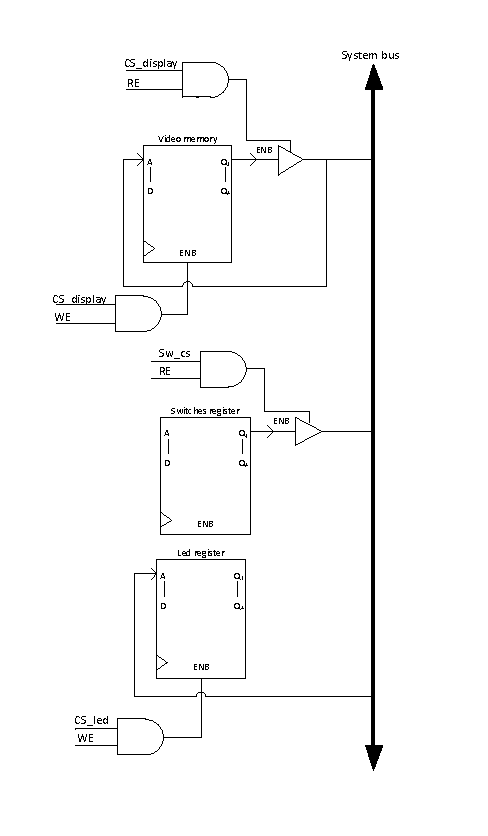
\epsfig{file=fig/system.eps, width=3.0in}
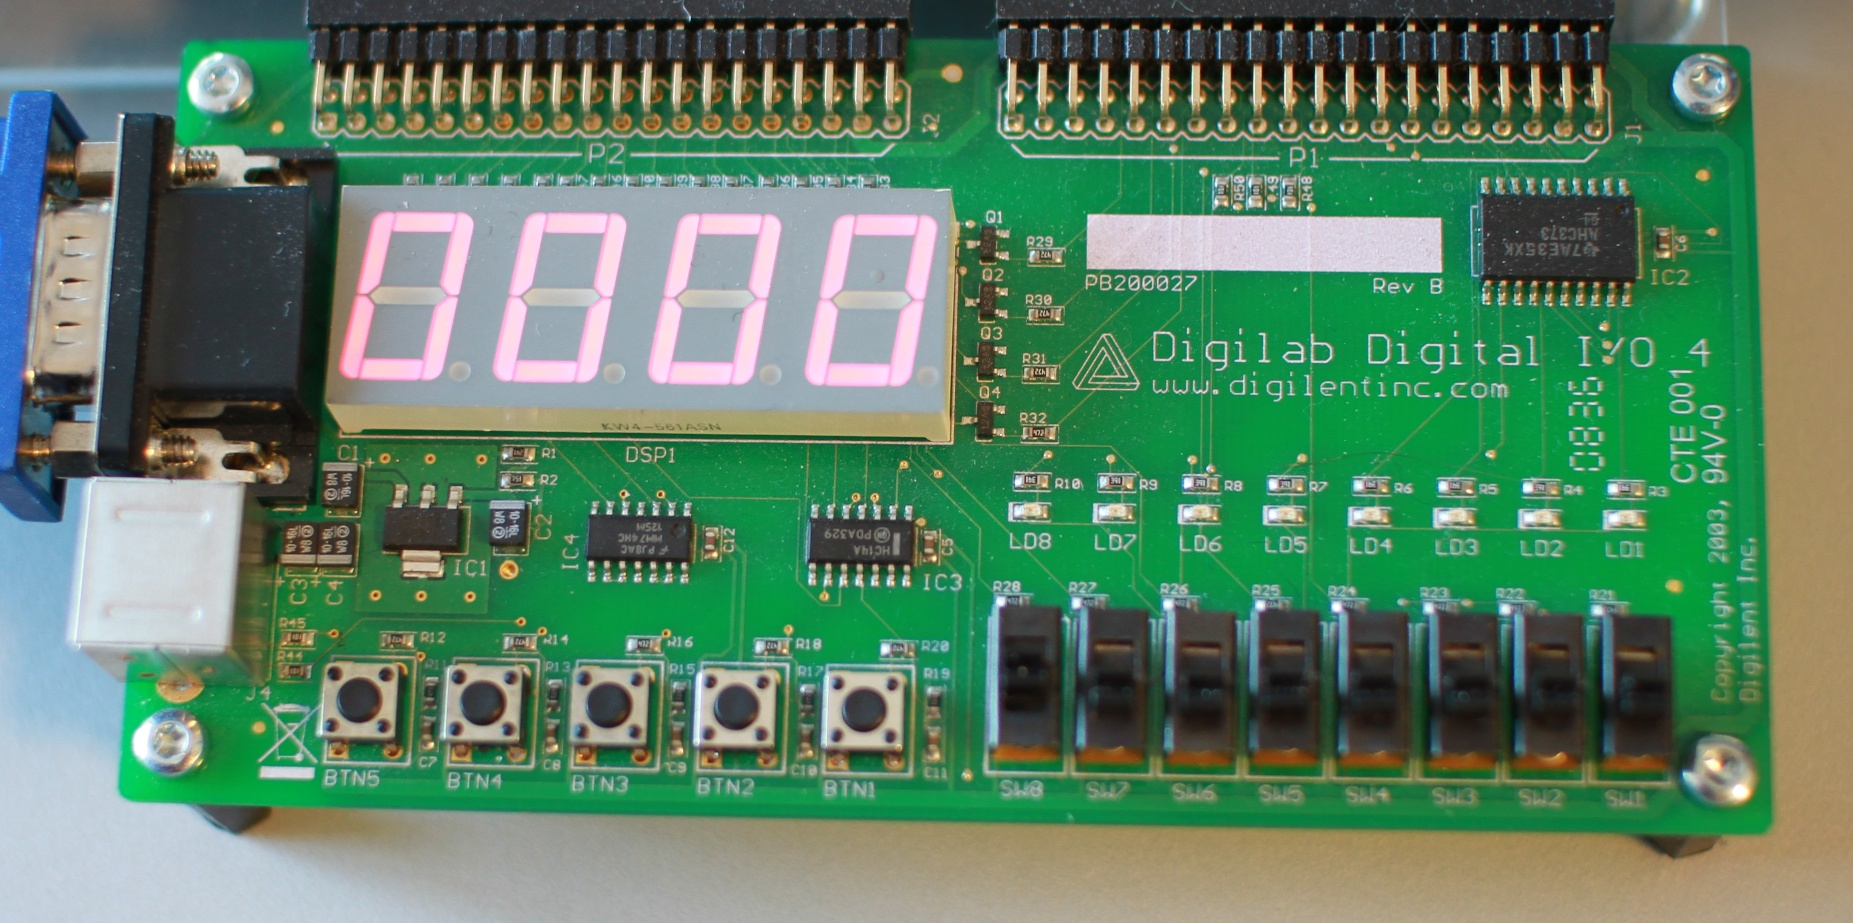
\includegraphics[scale=0.064]{img/DIO4Buttons.jpg} 
\caption{DIO4 Board}
\label{fig:dio4board}
\end{figure}

BTN1 is right, BTN2 left, BTN3 up and BTN4 is down.\\
The game can be reset at any point by colliding with hurdles or pressing the enter button on the FPGA board.

\section{Known bugs}
This section contains the bugs that we have identified, their severity and their status.
\subsection{Initial snake tail inconsistent}
When starting a new game, either at machine reset or when the snake dies, the tail follows an inconsistent linking leaving blank spaces for the first few game cycles. This is probably due to a bug in the way the snake body is generated in the "initialize\_snake" function.\\
The game works and renders fine after the first three cycles, and the bug does not affect gameplay.\\\\
Severity: Negligible\\
Status: Not fixed

\subsection{Snake stops on invalid button input}
When the user presses the btn5 or more than one button at once, the snake stops updating and the head becomes the tile rom index corresponding to the binary input on the buttons. The snake and the game continues if a valid button is pressed, but the graphics are incorrectly updated for the body elements.\\
This bug affects gameplay and is more severe as players often by accident press more than one button.

This bug was fixed late in the project period.

Severity: Important\\
Status: Fixed

\subsection{Score stops at 9}
When a user has reached a score of 10 or more the display is not updated with a valid value, but with the ASCII value of the score plus 30.

Severity: Essential to gameplay\\
Status: Not fixed

\section{Report distribution}
Kim Rostgaard Christensen
\begin{itemize}
	\item Report
	\begin{itemize}
		\item Design
		\item Known bugs
		\item Conclusion
		\item Discussion
	\end{itemize}
	\item Development
	\begin{itemize}
		\item LC-3 Computer
		\item Game logic
		\item Tile linking
	\end{itemize}
\end{itemize}

Morten Hillebo
\begin{itemize}
	\item Report
	\begin{itemize}
		\item Abstract
		\item Introduction
		\item Conclusion
		\item Discussion
		\item Requirements specification
		\item User manual
	\end{itemize}
	\item Development
	\begin{itemize}
		\item C functions
		\item Snake model
		\item Game initialization
		\item Tile map
	\end{itemize}
\end{itemize}


%Appendixes; Appendixes holds, for example, results or figures that are not
%relevant to place in the body of the report. Appendixes should generally be
%avoided and might not be read by the course staff.


\end{document}
